\scanpage{2}
\deleted{bien \unsure{distinguer|déterminé} $\bar D_{J,\alpha}$ de $\bar D_J$, cf. \unsure{9}}
\deleted{\diagram{\begin{tikzcd}
\bar U_{J',\alpha'} \arrow[r] \arrow[d] & \bar U_{J,\alpha} \arrow[r] \arrow[d] & \bar U \arrow[d] \\
U_{J',\alpha'} \arrow[r] & U_{J,\alpha} \arrow[r] & U
\end{tikzcd}}}

\diagram{\begin{tikzcd}[column sep=small]
D=U(\mathbb C)^{\sim} \arrow[rr] \arrow[dr,"\pi"'] && \widetilde U(\mathbb C)\deleted{\unsure{\ne U|=U}} \arrow[dl,"\hat\pi"] \\
& U(\mathbb C) &
\end{tikzcd}}
\[ \pi\subset G \]
\[
H_{\deleted{\unsure{u}}}=\bigl\{u\in G\mid \exists
\underset{\substack{\text{\unsure{ss=gr.|ss-gr.}}\\\text{d'indice fini}}}{\begin{gathered}\pi'\subset\pi\\[-.8ex]
\begin{tikzpicture}[x=1cm,y=1cm,baseline=0pt]\draw (0,.09) .. controls (-.04,-.01) and (-.01,-.05) .. (.10,-.05)--(1.25,-.05) .. controls (1.38,-.05) and (1.38,.03) .. (1.30,.09);\end{tikzpicture}\end{gathered}},\quad
\underset{\text{id.}}{\begin{gathered}\pi''\subset\pi\\[-.8ex]
\begin{tikzpicture}[x=1cm,y=1cm,baseline=0pt]\draw (0,.09) .. controls (-.04,-.01) and (-.01,-.05) .. (.10,-.05)--(1.25,-.05) .. controls (1.38,-.05) and (1.38,.03) .. (1.30,.09);\end{tikzpicture}\end{gathered}},
\quad\text{iso }v:D/\pi'\simeq D/\pi'',\quad\text{avec}
\]
\diagram{\begin{tikzcd}
D \arrow[r,"u"] \arrow[d,"p'"'] & D \arrow[d,"p''"] & \text{commutatif} \\
D/\pi' \arrow[r,"\substack{v\\\sim}"] & D/\pi'' &
\end{tikzcd}}

\uline{NB} On aura, pour $u,\pi',\pi'',v$ comme dessus un iso
\figure{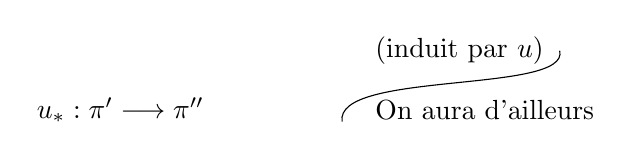
\begin{tikzpicture}
\node[anchor=west] (map) at (0,0) {$u_*:\pi'\longrightarrow\pi''$};
\node[anchor=west] (ins) at (4.3,.75) {\inserted{(induit par $u$)}};
\draw ([xshift=.08cm]ins.east) .. controls (6.9,.2) and (3.9,.5) .. (4,-.15);
\node[anchor=west] at (4.3,0) {On aura d'ailleurs};
\end{tikzpicture}}
$\pi'$ et $\pi''$ de $=$ indice dans $\pi$.
\margin{$u$ est déterminé par $v_*$}

\uline{NB} $v$ est connu quand on connaît $v_*$ (\uline{ces conditions}), et quand $v$ est connu, $u$ est connu \deleted{\unsure{aux}} mod multiplication \uline{\unsure{à|:} gauche} par un $\gamma\unsure{\in|+}\pi''$.

\margin{\diagram{\begin{tikzcd}[column sep=small]
& \pi & \\
\pi' \arrow[ur,phantom,"\tikz[baseline=-.5ex]{\node[rotate=-35,inner sep=0pt] {$\cup$};}" description] \arrow[rr,phantom,"\simeq" description] && \pi'' \arrow[ul,phantom,"\tikz[baseline=-.5ex]{\node[rotate=15,inner sep=0pt] {$\cup$};}" description]
\end{tikzcd}}
\[\pi_i'\simeq\pi_i''\]}
\margin{\[
p''u=vp'
\]
\[\deleted{p''u\gamma=}\]
\[p''(\gamma u)=(p''\gamma)u=p''u=vp')\]
\[\deleted{\pi\subset H}\]}

$H$ est un groupe $\supset\pi$, et $H/\pi$ (classes \unsure{à|:} droite) s'identifie à un sous-ens de \unsure{l'ens|l'un} des ``germes'' \uline{d'isom} \deleted{\unsure{des}} $H$-groupes d'indice \unsure{finis|fini} de $\pi$ de $=$ indice

$H_n=$ sous-ens de $H$ formé des $u$ pour lesquels on peut prendre $\pi',\pi''$ d'indice $n$.

$H_n$ est un \uline{ss-groupe}, et $\pi$ d'indice
\mspage{1}
